% !TEX encoding = UTF-8 Unicode
% $Header: /cvsroot/latex-beamer/latex-beamer/solutions/conference-talks/conference-ornate-20min.en.tex,v 1.6 2004/10/07 20:53:08 tantau Exp $

\documentclass{beamer}

\mode<presentation>
{
  \usetheme{Warsaw}
  % or ...

  \setbeamercovered{transparent}
  % or whatever (possibly just delete it)
  
  \setbeamertemplate{navigation symbols}{}
  
  \newcommand*\oldmacro{}%
  \let\oldmacro\insertshorttitle%
  \renewcommand*\insertshorttitle{%
    \oldmacro\hfill%
    \insertframenumber\,/\,\inserttotalframenumber}
}

\usepackage[utf8]{inputenc}
% or whatever

\usepackage{times}
\usepackage{multirow}
\usepackage[T1]{fontenc}
\usepackage[french]{babel}
\usepackage{graphicx}
\usepackage{CJKutf8}

\usepackage{eso-pic}
\usepackage{color}
\usepackage{tikz}
\usepackage{wasysym}

% Or whatever. Note that the encoding and the font should match. If T1
% does not look nice, try deleting the line with the fontenc.

%\title[Petit guide des bonnes pratiques pour la construction et la maintenance d'$\alpha$-extracteurs cosmiques à vacuité]
{}

\titlegraphic{\raisebox{2em}{}}

\author[Prologin]
{
\includegraphics{../prologin2016}}

\date
{}

\begin{document}

\definecolor{vert}{rgb}{0.07 0.54 0.07}


\begin{frame}
        \centering 
\includegraphics[width=0.9\linewidth]{../prologin2016} \\
        \vspace{1.5cm}
 	Guide des bonnes pratiques pour la construction et la
 	maintenance de tuyaux extracteurs cosmiques à vacuité
\end{frame}

\begin{frame}
    La simulation
\end{frame}

\begin{frame}
	\frametitle{Présentation}
	\begin{itemize}
        \item Confrontation 2 joueurs
        \item Tour par tour
        \item Récolter maximum d'énergie
	\end{itemize}
\end{frame}

\begin{frame}
	\frametitle{Site}
	\center{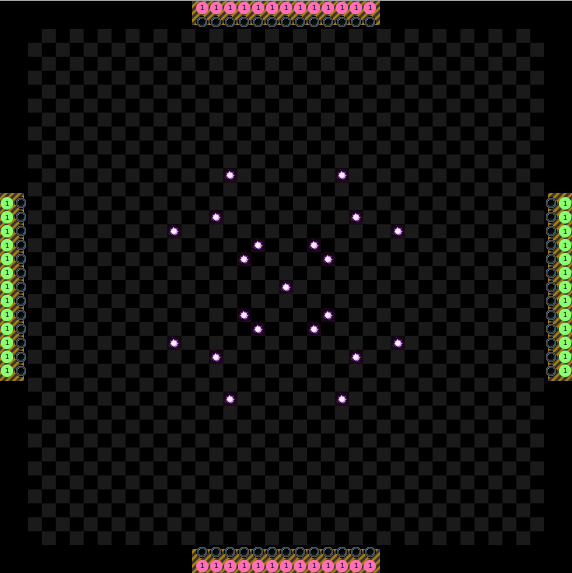
\includegraphics[width=7cm]{pictures/map}}
\end{frame}

\begin{frame}
	\frametitle{Pulsar}
    \begin{columns}[T]
        \begin{column}{.3\textwidth}
            
\includegraphics[width=3cm]{pictures/pulsar}
        \end{column}
        \begin{column}{.7\textwidth}
            \begin{itemize}
                \item Période de pulsation $T$
                \item Puissance d'émission $P$
                \item Nombre de pulsations restantes $R$
            \end{itemize}
        \end{column}
    \end{columns}
\end{frame}

\begin{frame}
	\frametitle{Tuyau}
    \begin{columns}[T]
        \begin{column}{.3\textwidth}
            
\includegraphics[width=3cm]{pictures/tuyau}
        \end{column}
        \begin{column}{.7\textwidth}
            \begin{itemize}
                \item Construit dans les zones vides
                \item Neutre
                \item Conduit le plasma
            \end{itemize}
        \end{column}
    \end{columns}
\end{frame}

\begin{frame}
	\frametitle{Plasma}
    \begin{columns}[T]
        \begin{column}{.3\textwidth}
            
\includegraphics[width=3cm]{pictures/emission}
        \end{column}
        \begin{column}{.7\textwidth}
            \begin{itemize}
                \item Ressource convoitée
                \item Émis par les pulsars
                \item Acheminé aux bases par des tuyaux
                \item Disparaît si non relié à une base
                \item Se déplace vers la base la plus proche
            \end{itemize}
        \end{column}
    \end{columns}
\end{frame}

\begin{frame}
	\frametitle{Déplacement du plasma}
    \begin{columns}[T]
        \begin{column}{.5\textwidth}
            \center{Se dirige vers la base la plus proche} \\
            \center{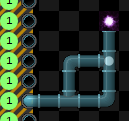
\includegraphics[width=3cm]{pictures/before_division}}
        \end{column}
        \begin{column}{.5\textwidth}
            \center{Se divise en cas d'égalité vers plusieurs directions} \\
            \center{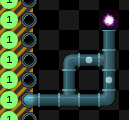
\includegraphics[width=3cm]{pictures/after_division}}
        \end{column}
    \end{columns}
\end{frame}

\begin{frame}
	\frametitle{Base}
    \begin{columns}[T]
        \begin{column}{.3\textwidth}
            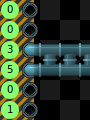
\includegraphics[width=3cm]{pictures/aspiration}
        \end{column}
        \begin{column}{.7\textwidth}
            \begin{itemize}
                \item Case de récolte du plasma
                \item Peuvent être boostées et mieux aspirer
                \item Points d'aspirations transférables
                \item Entre 0 et 5 points d'aspiration par case
            \end{itemize}
        \end{column}
    \end{columns}
\end{frame}

\begin{frame}
    \frametitle{Super-Tuyau™}
    \begin{columns}[T]
        \begin{column}{.3\textwidth}
            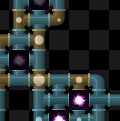
\includegraphics[width=3cm]{pictures/super-tuyau}
        \end{column}
        \begin{column}{.7\textwidth}
            \begin{itemize}
                \item Amélioration d'un tuyau existant
                \item Plus résistant
                \item Le plasma se déplace de deux cases
            \end{itemize}
        \end{column}
    \end{columns}
\end{frame}

\begin{frame}
    \frametitle{Débris}
    \begin{columns}[T]
        \begin{column}{.3\textwidth}
            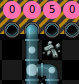
\includegraphics[width=3cm]{pictures/destruction}
        \end{column}
        \begin{column}{.7\textwidth}
            \begin{itemize}
                \item Restes d'un tuyau détruit
                \item Zone inconstructible
                \item Peut uniquement être déblayé
            \end{itemize}
        \end{column}
    \end{columns}
\end{frame}
\begin{frame}
	\frametitle{Points d'actions}
    100 tours :
	\begin{columns}[T]
        \begin{column}{.65\textwidth}
            \begin{itemize}
	            \item[+] commencer un tour
	            \item[\alert{--}] construire un tuyau
	            \item[\alert{--}] améliorer un tuyau
	            \item[\alert{--}] déplacer la puissance d'aspiration
	            \item[\alert{--}] détruire un tuyau/Super Tuyau™
	            \item[\alert{--}] déblayer un tuyau détruit
	        \end{itemize}
        \end{column}
        \begin{column}{.35\textwidth}
            \begin{itemize}
                \item[] 4
	            \item[] 1
	            \item[] 1
	            \item[] 0 $\rightarrow$ 1
                \item[] 3/4 (+ 2 plasmas)
	            \item[] 2
            \end{itemize}
        \end{column}
    \end{columns}
    \vspace{0.5cm}
    Celui qui a récolté le plus de plasma gagne !
\end{frame}

\begin{frame}
    \frametitle{Questions}
    Posez vos questions sur le sujet de la finale
\end{frame}

\begin{frame}
    \frametitle{Tournois intermédiaires}
    \begin{itemize}
        \item Samedi 15~h~42 (tournoi test)
        \item Samedi 17~h~42
        \item Samedi 23~h~42
        \item Dimanche 5~h~42
        \item Dimanche 11~h~42
        \item Dimanche 17~h~42
        \item Lundi 00~h~42 (tournoi final)
    \end{itemize}
\end{frame}

\begin{frame}
    \frametitle{Conférences}
    \begin{itemize}
        \item \textbf{Samedi 9~h~50} Benjamin Jean : Open Law et Open Source Summit
        \item \textbf{Samedi 16~h~00} Jill-Jênn Vie : \begin{CJK}{UTF8}{min}「アルゴのせい、アルゴのおかげ」\end{CJK} (tryalgo : pros and cons)
        \item \textbf{Lundi 11~h~45} Xavier Garrigue : Apycat
    \end{itemize}
\end{frame}

\begin{frame}
    \frametitle{Fin}
    Bonne finale !
\end{frame}

\end{document}
